% ======================= Pre-Amble =========================

\documentclass[11pt, oneside]{article}   	% use "amsart" instead of "article" for AMSLaTeX format 
                     						%imports package {article} and specify option(s) [11pt, oneside]
\usepackage{geometry}                		% See geometry.pdf to learn the layout options. There are lots.                                        

\geometry{letterpaper}                   		% ... or a4paper or a5paper or ... 
%\geometry{landscape}                		% Activate for rotated page geometry

\usepackage[parfill]{parskip}    		        % Activate to begin paragraphs with an empty line rather than an indent

\usepackage[hidelinks]{hyperref}                % Allows for clickable references

%American Mathematics Society packages
\usepackage{amsmath}	   %math
\usepackage{amssymb}       %symbols
\usepackage{amsthm}          %theorems

%Graphics
\usepackage{graphicx, subcaption}
\usepackage[usenames, dvipsnames]{color}     % font colour:    \textcolor{<colour>}{text}
      									%highlight text:  \colorbox{<color>}{text}
									
									%list of colours: https://www.sharelatex.com/learn/Using_colours_in_LaTeX

%Images		                
\graphicspath{ {images/} }                          %directory that your images are located in within your current directory
	

%Footnote Spacing
\setlength{\footnotesep}{0.4cm}                  %specify spacing b/w footnotes
\setlength{\skip\footins}{0.6cm}                    % space b/w footnotes and textbody

%Table
\usepackage[none]{hyphenat}                    % Stops breaking-up words in a table (i.e. no hyphens)                                                             

\usepackage{array}   
\newcolumntype{x}[1]{>{\centering\let\newline\\\arraybackslash\hspace{0pt}}p{#1}}       %center fixed column width: x{<len>}                      
\newcolumntype{$}{>{\global\let\currentrowstyle\relax}}                                                   % let us apply things (e.g. bold/italicize) to entire row            
\newcolumntype{^}{>{\currentrowstyle}}
\newcommand{\rowstyle}[1]{\gdef\currentrowstyle{#1} #1\ignorespaces}

%Bibliography
\usepackage[numbers,sort&compress]{natbib}   %for multiple references: sorts  (i.e. [1,2] NOT [2, 1] )
                                           				  %                                     compresses (i.e. [1-3] )
\usepackage[nottoc]{tocbibind}                            %add bibliography to table of contents

%Bullets
\usepackage{enumerate}     %specify type of enumeration: \being{enumerate}[<type of enumeration>]

%QED
\newcommand*{\QEDA}{\hfill\ensuremath{\blacksquare}}         %make qed filled square:    \QEDA
%\newcommand*{\QEDB}{\hfill\ensuremath{\square}}               %make qed empty square: \QEDB 

%Header and Footer
\usepackage{fancyhdr}
\usepackage{lastpage}      %ensures you can reference LastPage (i.e. Page 2 of 10)

%Diagrams
\usepackage[latin1]{inputenc}
\usepackage{tikz}
\usepackage{tkz-berge}
\usetikzlibrary{shapes,arrows}

%Miscellaneous
\usepackage{dirtytalk}    %quotations: use \say  

\usepackage{caption}
\captionsetup[figure]{labelfont=bf}    %make figure labels boldface
\captionsetup[table]{labelfont=bf}     %make table labels boldface


%=========== Header & Footer =========================

\pagestyle{fancy}
\lhead{Stephanie Knill} 		% controls the left corner of the header
\chead{} 					% controls the center of the header
\rhead{} 					% controls the right corner of the header
\lfoot{} 					% controls the left corner of the footer
\cfoot{Page~\thepage\ of \pageref{LastPage}} 				% controls the center of the footer
												%Page~\thepage\  if just want Page x
\rfoot{}			 		% controls the right corner of the footer
\renewcommand{\headrulewidth}{0.4pt}
\renewcommand{\footrulewidth}{0.4pt}

\setlength{\headsep}{0.3in}		%space b/w page header and body

% ======================== Document ======================
\begin{document}

\title{MATH 442 --- Assignment 4 \\
\line(1,0){360} \\              %(slope x, y){length of line}
}
\author{
Stephanie Knill \\
54882113 \\
Due: January 28, 2015}

\date{}                   % Activate:  display a given date (e.g. {August 4} ) or no date (empty {} )
                                    %No activate: display current date
\maketitle


\thispagestyle{empty}                   %Remove header from this (first) page. Change empty -> plain to keep numbering

% ================= Questions ================

\section*{Question 19}

\begin{enumerate}[\quad (a)]

	\item A connected graph $G$ that is Hamiltonian but not Eulerian can be seen in Figure~\ref{H not E}.
	\begin{figure}[h]
            %Latex Documentation: http://www.texample.net/tikz/examples/tkz-berge/
            \centering
            
            \begin{tikzpicture}[scale=0.75,transform shape]
              \Vertex[x=0,y=0]{D}
              \Vertex[x=0,y=3]{A}
              \Vertex[x=3,y=0]{C}
              \Vertex[x=3,y=3]{B}
              \Vertex[x=1.5,y=1.5]{E}
            
              \tikzstyle{LabelStyle}=[fill=white,sloped]
              %Edges bend left
              \tikzstyle{EdgeStyle}=[bend left]		%\Edge[label=$120$](A)(B)  %if want to label the edge
                  			
              %Edges bend right
              \tikzstyle{EdgeStyle}=[bend right]
            
              %Edges straight
              \tikzstyle{EdgeStyle}=[]
                  \Edge(A)(B)
                  \Edge(B)(C)
                  \Edge(C)(D)    
                  \Edge(D)(A)
                  \Edge(A)(E)
                  \Edge(B)(E)
                  \Edge(C)(E)
                  \Edge(D)(E)
            \end{tikzpicture}
            
            \caption{A connected graph that is Hamiltonian but not Eulerian.}
            \label{H not E}
          \end{figure}
          
          Here we have 4 odd degree vertices, thus it is not Eulerian. However, we have that $deg(A)=deg(B)=deg(C)=deg(D)=3$ and $deg(E)=4$. Since each vertex has a degree greater than half the number of vertices $n=5$, then by Ore's Theorem the graph $G$ is Hamiltonian.
          
          \item A connected graph $G'$ that is Eulerian but not Hamiltonian can be seen in Figure~\ref{E not H}.
          
          \begin{figure}[h]
            %Latex Documentation: http://www.texample.net/tikz/examples/tkz-berge/
            \centering
            
            \begin{tikzpicture}[scale=0.75,transform shape]
              \Vertex[x=0,y=0]{D}
              \Vertex[x=0,y=3]{A}
              \Vertex[x=3,y=0]{C}
              \Vertex[x=3,y=3]{B}
              \Vertex[x=1.5,y=1.5]{E}
            
              \tikzstyle{LabelStyle}=[fill=white,sloped]
              %Edges bend left
              \tikzstyle{EdgeStyle}=[bend left]		%\Edge[label=$120$](A)(B)  %if want to label the edge
                  			
              %Edges bend right
              \tikzstyle{EdgeStyle}=[bend right]
            
              %Edges straight
              \tikzstyle{EdgeStyle}=[]
                  \Edge(A)(B)
                  \Edge(C)(D)    
                  \Edge(A)(E)
                  \Edge(B)(E)
                  \Edge(C)(E)
                  \Edge(D)(E)
            \end{tikzpicture}
            
            \caption{A connected graph that is Eulerian but not Hamiltonian.}
            \label{E not H}
          \end{figure}

	Here we have no odd degree vertices, thus it is Eulerian. Although our graph $G'$ fails both Ore's and Dirac's, this is not sufficient to conclude that it is not Hamiltonian. We can see, however, that vertex $E$ is a cut-vertex. Therefore in order to travel to and from each half of the graph, we will need to traverse vertex $E$ twice. Thus we can conclude that $G'$ is not Hamiltonian.

\end{enumerate} 


\section*{Question 20}

{\textbf{Proof:} In every connected graph $G$ we can always find a sequences of edges that start at a vertex and return to it at the end and traverses every edge \textit{twice}.

Let $G$ be any connected graph and $G'$ the same graph but with twice the number of edges joining any two vertices. Since visiting each edge twice is equivalent to doubling the number of edges in our graph and conducting an Euler tour, then if we can show that $G'$ is Eulerian, we are done.

When we doubled the number of edges emerging from each vertex, we also doubled the degree of every vertex in $G'$. Since each vertex is now of even degree, we can conclude that $G'$ is Eulerian.  \QEDA


\section*{Question 21}

{\textbf{Proof:} Every Eulerian graph that is simple with an odd number of vertices greater than 1 contains at least 3 vertices of the same degree.

\textbf{Proof by Contradiction}

Assume that for a simple Eulerian graph with an odd number of vertices greater than 1, there \textit{does not} exist 3 vertices of the same degree.


For a graph of $n=3, 5, 7, \ldots$ vertices, we can only have two vertices of degree 2, two vertices of degree 4, ... , two vertices of degree $n-1$. Thus the set of all possible vertex degrees in a graph of $n$ vertices has length of $n-1$. However, we have not assigned a degree to the $n$-th vertex. Since the max number of degrees in a simple graph of $n$ vertices is $n-1$, we cannot assign a degree of $n+1$ to our final vertex. Therefore, we must have at least 3 vertices of the same degree, thereby contradicting our initial assumption. \QEDA


\section*{Question 22}

\textbf{Proof:} Let $G$ be a Hamiltonian graph and let $S$ be any set of $k$ vertices in $G$. Then the graph $G - S$ has at most $k$ components.

Let us first imagine our Hamiltonian graph as a cycle graph, where each vertex is of degree 2.

Since we have a Hamiltonian cycle, the deletion of the first vertex will not result in another component, thus we have 1 component for $k=1$ deleted vertices. However, since we no longer have a Hamiltonian cycle, the possibility of a cut-vertex now exists. In the case where the next deleted vertex is a cut-set vertex, then we will have 2 components for $k=2$. Otherwise, we will either the same number or less (we can have less components if the deleted vertex was an isolated vertex) components. Thus with each successive deletion of a vertex, we can at most break our graph into 1 more components. Therefore we can conclude that in a cycle graph,  the number of vertices deleted $k$ will be greater than or equal to the number of components of $G - S$.

Now let us lift our restriction on the Hamiltonian graph being a cycle graph. Since any edges outside of the Hamiltonian cycle will only increase the graph's connectivity, then this will only increase the possibility of the deleted vertex not being a cut-set vertex. Thus the graph $G-S$ having at most $k$ components holds true for all Hamiltonian graphs. \QEDA


\section*{Question 23}

\textbf{Proof:} We will show by induction that for all $n \geq 2$, $Q_n$ is Hamiltonian.

	\textbf{\textit{Base Case:}} for $n=2$, we have the 2-dimensional hypercube $Q_2$ (Figure~\ref{Q2})
	
	\begin{figure}[h]
            %Latex Documentation: http://www.texample.net/tikz/examples/tkz-berge/
            \centering
            
            \begin{tikzpicture}[scale=0.75,transform shape]
              \Vertex[x=0,y=0]{00}
              \Vertex[x=0,y=3]{10}
              \Vertex[x=3,y=0]{01}
              \Vertex[x=3,y=3]{11}
            
              \tikzstyle{LabelStyle}=[fill=white,sloped]
              %Edges bend left
              \tikzstyle{EdgeStyle}=[bend left]		%\Edge[label=$120$](A)(B)  %if want to label the edge
                  			
              %Edges bend right
              \tikzstyle{EdgeStyle}=[bend right]
            
              %Edges straight
              \tikzstyle{EdgeStyle}=[post]
                  \Edge(00)(10)
                  \Edge(10)(11)
                  \Edge(11)(01)    
                  \Edge(01)(00)
            \end{tikzpicture}
            
            \caption{A hypercube $Q_2$.}
            \label{Q2}
          \end{figure}
          
          and we can see that $00 \rightarrow 10 \rightarrow 11 \rightarrow 01 \rightarrow 01$ is indeed a Hamiltonian cycle.
	
	\textit{\textbf{Induction Step:}} assume that a $k$-dimensional hypercube $Q_{k}$ has a Hamiltonian cycle.
	
	 For notation purposes, let a sequence of 0's of length $m$ be denoted by $0^m$ and a sequence of 1's of length $m$ be denoted by $1^m$ (For example, $0^m$ where $m=3$ would be the vertex 000). Since there must exist a Hamiltonian cycle in $Q_k$, then we know there exists a Hamiltonian cycle in $0v$ and $1v$, where $v$ is the set of all possible permutations of 0's and 1's of length $k$. Thus, if we can connect these two Hamiltonian cycles without visiting any vertex more than once, than we will have a Hamiltonian cycle in $Q_{k+1}$.
	
	 Without loss of generality, let us start at vertex $0^{k+1}$. Now let us go for a walk through all the vertices labelled $0v$, where we must end on a vertex that is adjacent to $0^n$. We will denote this vertex as $0u$.
	
	Now let us cross over to the other half of the graph, which we know also contains a Hamiltonian cycle. We do this by walking along the edge connecting $0u$ to $1u$. From here, let us continue our walk by traversing all vertices labeled $1v$. Our final point in this path is the vertex $10^{k}$, as it is adjacent to our starting point $0^{k+1}$.
	
	At this point we have now traversed every vertex in our graph $Q_{k+1}$ without repetition. Taking our last step from $10^{k}$ to $0^{k+1}$ closes the path and our Hamiltonian cycle in $Q_{k+1}$ is complete.
	
	\textit{\textbf{Conclusion:}} By the principle of induction, we can conclude that a Hamiltonian cycle exists in $Q_n$ for all $n \geq 2$. \QEDA
	
	
	\begin{figure}[h]
            %Latex Documentation: http://www.texample.net/tikz/examples/tkz-berge/
            \centering
            
            \begin{tikzpicture}[scale=0.75,transform shape]
              \Vertex[L=$0u$, x=0,y=0]{0u}
              \Vertex[L=$0^k$, x=0,y=4]{0k}
              \Vertex[L=$1u$, x=4,y=0]{1u}
              \Vertex[L=$10^k$, x=4,y=4]{10k}
              
              \Vertex[L=$0v$, x=-3,y=2]{0v}
              \Vertex[L=$1v$, x=7,y=2]{1v}
            
              \tikzstyle{LabelStyle}=[fill=white,sloped]
              %Edges bend left
              \tikzstyle{EdgeStyle}=[bend left]		%\Edge[label=$120$](A)(B)  %if want to label the edge
                 		
              %Edges bend right
              \tikzstyle{EdgeStyle}=[post, dashed, bend right]	
		\Edge(0v)(0u)
		\Edge(1v)(10k)	
	      \tikzstyle{EdgeStyle}=[dashed, bend right]	
	      	\Edge(0k)(0v)
		\Edge(1u)(1v)
            
              %Edges straight
              \tikzstyle{EdgeStyle}=[post]
                  \Edge(0u)(1u)
                  \Edge(10k)(0k)
            \end{tikzpicture}
            
            \caption{A Hamiltonian cycle $0^k \rightarrow 0u \rightarrow 1u \rightarrow 10^k \rightarrow 0^k$, for the hypercube $Q_{k+1}$.}
            \label{Qk+1}
          \end{figure}
	
	
\cleardoublepage
\section*{Question 24}

For the given four cubes problem where each cube is coloured Red (R), Blue (B), Green (G) and Yellow (Y), let us express each cube as a graph having a vertex for each colour and an edge between two vertices if the colours are opposite on the cube (Figure \ref{4 cubes}).
    \begin{figure}[h]
    \centering
    
    \begin{subfigure}[b]{0.2\columnwidth}             
    \centering
      \begin{tikzpicture}[scale=0.75,transform shape]
      	\Vertex[x=0,y=0]{G}
     	\Vertex[x=0,y=2]{R}
     	\Vertex[x=2,y=0]{Y}
     	\Vertex[x=2,y=2]{B}

      \tikzstyle{EdgeStyle}=[red]			%\Edge[label=$120$](A)(B)  %if want to label the edge
    		\Edge(R)(G)
		\Edge(G)(B)
		\Edge(R)(Y)
      \end{tikzpicture}
      \caption{Cube 1}
      \label{A}
    \end{subfigure}
    \begin{subfigure}[b]{0.2\columnwidth}
      \centering
      \begin{tikzpicture}[scale=0.75,transform shape]
      	\Vertex[x=0,y=0]{G}
     	\Vertex[x=0,y=2]{R}
     	\Vertex[x=2,y=0]{Y}
     	\Vertex[x=2,y=2]{B}
    
     	 \tikzstyle{EdgeStyle}=[blue]			%\Edge[label=$120$](A)(B)  %if want to label the edge
        		\Edge(R)(G)
    		\Edge(G)(B)
    		\Edge(R)(Y)
      \end{tikzpicture}
      \caption{Cube 2}
    \end{subfigure}
    \begin{subfigure}[b]{0.2\columnwidth}
      \centering
      \begin{tikzpicture}[scale=0.75,transform shape]
      	\Vertex[x=0,y=0]{G}
     	\Vertex[x=0,y=2]{R}
     	\Vertex[x=2,y=0]{Y}
     	\Vertex[x=2,y=2]{B}
    
	%Loop edge
       \tikzstyle{EdgeStyle}=[green]
	 \Loop[dist=2cm, dir=NOEA](Y)		%NO = north, EA = east
    
    	%Edges straight
    	\tikzstyle{EdgeStyle}=[green]			%\Edge[label=$120$](A)(B)  %if want to label the edge
        		\Edge(R)(G)
    		\Edge(Y)(B)
    	\end{tikzpicture}
    	\caption{Cube 3}
    \end{subfigure}
        \begin{subfigure}[b]{0.2\columnwidth}
      \centering
      \begin{tikzpicture}[scale=0.75,transform shape]
      	\Vertex[x=0,y=0]{G}
     	\Vertex[x=0,y=2]{R}
     	\Vertex[x=2,y=0]{Y}
     	\Vertex[x=2,y=2]{B}
    	
    %Loop edge
       \tikzstyle{EdgeStyle}=[yellow]
	 \Loop[dist=2cm, dir=SOEA](B)		%SO = south, EA = east
    
    	%Edges straight
    	\tikzstyle{EdgeStyle}=[yellow]			%\Edge[label=$120$](A)(B)  %if want to label the edge
        		\Edge(R)(B)
    		\Edge(Y)(G)
    	\end{tikzpicture}
    	\caption{Cube 4}
    \end{subfigure}
   
    
    \caption{Four cube problem expressed graphically}
    \label{4 cubes}
    \end{figure}


Next, we will superimpose these graphs (Figure \ref{superimposition}).

  \begin{figure}[h]
    \centering
    \begin{tikzpicture}[scale=0.75,transform shape]
      	\Vertex[x=0,y=0]{G}
     	\Vertex[x=0,y=4]{R}
     	\Vertex[x=4,y=0]{Y}
     	\Vertex[x=4,y=4]{B}
    
    %Cube1: Red
	\tikzstyle{EdgeStyle}=[red]			
    		\Edge(R)(G)
		\Edge(G)(B)
		\Edge(R)(Y)
    %Cube2: Blue
     	\tikzstyle{EdgeStyle}=[blue]			
	\tikzstyle{EdgeStyle}=[bend right, blue]
	        	\Edge(R)(G)
		\Edge(G)(B)
    		\Edge(Y)(R)	
    %Cube3: Green
	\tikzstyle{EdgeStyle}=[green]
		 \Loop[dist=2cm, dir=NOEA](Y)		
	\tikzstyle{EdgeStyle}=[bend left, green]			
        		\Edge(R)(G)
	\tikzstyle{EdgeStyle}=[green]
    		\Edge(Y)(B)
    %Cube4: Yellow	
        \tikzstyle{EdgeStyle}=[yellow]
	 	\Loop[dist=2cm, dir=SOEA](B)		
    	\tikzstyle{EdgeStyle}=[yellow]			
        		\Edge(R)(B)
    		\Edge(Y)(G)
		
		
    \end{tikzpicture}  
    \caption{Superimposed graph of the four cubes.}
    \label{superimposition}
    \end{figure}

From here, we must find two subgraphs: one that will tell us the front and back colours of the stack; the other will tell us the left and right colours of the stack. However, these will be subject to 3 conditions:

\begin{enumerate}
	\item Each subgraph has an edge from each cube
	\item The subgraphs have no edge in common
	\item Each vertex is of degree 2
\end{enumerate}

Looking at these conditions, we will not be able to use either of the loops in Cube 3 or Cube 4. Since any vertex with a loop is of degree 2, connecting this vertex to the rest of the subgraph would violate our third condition. Thus we must use the two remaining edges in Cubes 3 and 4. Forcing these edges yields two cases (Figure \ref{Cases}):
\cleardoublepage

    \begin{figure}[h]           
    \centering
    \begin{subfigure}[b]{0.45\columnwidth}
    	\centering
     	 \begin{tikzpicture}[scale=0.75,transform shape]
      		\Vertex[x=0,y=0]{G}
     		\Vertex[x=0,y=2]{R}
     		\Vertex[x=2,y=0]{Y}
     		\Vertex[x=2,y=2]{B}
		
		\Vertex[L=G, x=4,y=0]{G2}
     		\Vertex[L=R, x=4,y=2]{R2}
     		\Vertex[L=Y, x=6,y=0]{Y2}
     		\Vertex[L=B, x=6,y=2]{B2}
    
    		\tikzstyle{EdgeStyle}=[green]		
        			\Edge(R)(G)
			\Edge(B2)(Y2)
		\tikzstyle{EdgeStyle}=[yellow]		
        			\Edge(G)(Y)
			\Edge(R2)(B2)
    	\end{tikzpicture}
    	\caption{Case 1}
    \end{subfigure}
    \begin{subfigure}[b]{0.45\columnwidth}
     	\centering
    	\begin{tikzpicture}[scale=0.75,transform shape]
      		\Vertex[x=0,y=0]{G}
     		\Vertex[x=0,y=2]{R}
     		\Vertex[x=2,y=0]{Y}
     		\Vertex[x=2,y=2]{B}
		
		\Vertex[L=G, x=4,y=0]{G2}
     		\Vertex[L=R, x=4,y=2]{R2}
     		\Vertex[L=Y, x=6,y=0]{Y2}
     		\Vertex[L=B, x=6,y=2]{B2}

    		\tikzstyle{EdgeStyle}=[green]		
        			\Edge(R)(G)
			\Edge(B2)(Y2)
		\tikzstyle{EdgeStyle}=[yellow]		
        			\Edge(G2)(Y2)
			\Edge(R)(B)
    	\end{tikzpicture}
    	\caption{Case 2}
    \end{subfigure}
   
    \caption{Two cases for the subgraphs, each using a different combination of the forced green and yellow edges.}
    \label{Cases}
    \end{figure}
    
    
In each case, if we can add the red (Cube 1) and blue (Cube 2) edges such that all three conditions hold true, then we have found a solution to our four cube problem. Let us examine the first case. Here, there is already an edge connecting vertex $R$ to vertex $G$, so we cannot use the same edge in our red and blue cubes. Since Cube 1 and Cube 2 have identical graphs, then without loss of generality we will add a red edge from vertex $R$ to vertex $Y$ and a blue edge from vertex $G$ to vertex $B$ in the first subgraph. However, this makes vertex $G$ have a degree of 3. Since this violates the third condition, there is no solution to the four cube problem in our first case.

Similarly in the second case, adding the remaining two pairs of red and blue edges to the first subgraph will result in at least one vertex being of degree 3. Therefore we can conclude there is no solution to this four cube problem. \QEDA

\end{document} 